\chapter{Implementação} 
\label{ch:IM}

Neste capítulo será demonstrado em detalhes o procedimento da aplicação de desenvolvimento de produto como anteriormente apresentado, 
com 9 etapas que expandem o modelo de \citeonline{Lawrence2019cucumber} para adaptá-lo ao produto em questão.

\section{\textbf{Etapa 1: Descrição das histórias de usuário}}
A etapa inicial do Desenvolvimento Orientado por Comportamento (BDD) consiste na definição das funcionalidades a serem implementadas por meio de histórias de usuário. 
Nessa fase, a perspectiva do usuário — ou da pessoa que se beneficia da funcionalidade — deve ser o foco principal. Essa abordagem é um dos pilares fundamentais do BDD, 
pois garante que o produto desenvolvido entregue valor real ao usuário final.

Portanto, no contexto deste trabalho que trata do sistema de travamento de portas veicular, serão consideradas implementações práticas amplamente adotadas pela 
indústria automotiva como base para as histórias de usuário criadas.

O travamento e destravamento remoto das portas, acionado por meio da chave com controle remoto ou até mesmo via celular, permite que todas as portas do veículo sejam 
travadas ou destravadas à distância, sem a necessidade de inserção da chave na fechadura \cite{bosch2022handbook}. Esse caso de uso mais simples é vastamente presente 
em veículos de diversas montadoras e pode ser capturado por meio de duas histórias de usuário:

\begin{itemize}
    \item Como dono de um veículo automotivo, quero travar todas as portas do meu carro utilizando o botão de travamento, para que eu possa mantê-lo seguro contra furtos e impedir o acesso de pessoas não autorizadas;
    \item Como dono de um veículo automotivo, quero destravar todas as portas do meu carro utilizando o botão de destravamento, para que eu possa acessá-lo.
\end{itemize}

Além disso, outra funcionalidade que é também vastamente presente é a indicação da confirmação do travamento ou destravamento das portas, que normalmente utiliza um 
sinal visual com os faróis do carro, assim como descrito por \citeonline{vwLocking}. A seguinte história de usuário será implementada para capturar essa funcionalidade:

\begin{itemize}
    \item Como dono de um veículo automotivo, quero receber uma indicação clara sempre que o travamento ou destravamento das portas ocorrer, para que eu tenha certeza do estado de segurança do meu carro.
\end{itemize}

Em alguns veículos como os da Volkswagen \cite{vwLocking}, há uma funcionalidade que permite destravar as portas sem a necessidade de usar a chave, desde que ela 
esteja próxima ao veículo. O sistema \textit{Keyless Access} possibilita que, ao interagir com as maçanetas das portas, o motorista possa destravar ou travar o carro sem 
precisar pressionar o botão no controle.

Esse recurso é útil em situações cotidianas, como quando o motorista deseja entrar no carro enquanto a chave está, por exemplo, no bolso. Embora o processo 
tradicional exija que o usuário retire a chave do bolso, pressione o botão de destravamento e, em seguida, guarde-a novamente, o uso do \textit{Keyless Access} simplifica 
essa sequência. A diferença é pequena — apenas alguns segundos de tempo —, porém a implementação de uma funcionalidade que elimina etapas desnecessárias torna a 
experiência mais prática, especialmente considerando que esse mesmo uso será repetido diversas vezes ao longo do dia.

O manual do veículo \textbf{ID.4} descreve funcionalidades adicionais, como o travamento das portas ou o destravamento total do veículo ao se interagir duas vezes com a maçaneta. 
No entanto, para fins de simplificação, este trabalho irá considerar apenas o cenário básico de destravamento de uma única porta — especificamente, aquela com a 
qual o usuário interage. Com base nisso, a seguinte história de usuário é adotada:

\begin{itemize}
    \item Como dono de um veículo automotivo, quero que a porta destrave automaticamente ao tentar abri-la com a chave em minha posse, para que eu possa acessar o veículo de forma mais rápida e conveniente.
\end{itemize}

Por fim, será implementada mais uma história de usuário, também baseada em funcionalidades descritas no manual do proprietário. Trata-se de um recurso que realiza o 
travamento automático do veículo após um determinado período de tempo, ativado em diferentes situações. Neste trabalho, a funcionalidade implementada será especificamente 
aquela em que o travamento automático é causado para evitar o destravamento não intencional.

Considerando que o usuário deseja manter seu veículo seguro contra furtos, garantir que ele permaneça travado é fundamental. Por esse motivo, identificar uma possível 
destrava indevida possui valor semelhante ao travamento convencional. A lógica adotada para essa funcionalidade depende de como o sistema reconhece a não intenção 
do motorista, o que deve ser inferido com base na interação do usuário com o veículo. Isso será definido na sessão do mapeamento de exemplos da história em questão, 
na próxima etapa.

Essa funcionalidade será capturada pela seguinte história de usuário:

\begin{itemize}
    \item Como dono de um veículo automotivo, quero que as portas sejam re-travadas automaticamente caso o carro seja destravado sem intenção, para que o veículo permaneça seguro contra acessos não autorizados.
\end{itemize}

\section{\textbf{Etapa 2: Mapeamento de exemplos}}
As histórias definidas na etapa anterior têm o papel de estabelecer um escopo claro da funcionalidade em discussão, garantindo que toda a equipe compreenda de forma 
alinhada o incremento de produto que está sendo proposto. Essa clareza é essencial para a etapa de mapeamento de exemplos, na qual ocorrem discussões colaborativas 
com pessoas de diferentes áreas.

É fundamental que todos os membros da equipe estejam cientes da ideia proposta e do valor que ela gera, pois isso permite um engajamento mais efetivo nas conversas. 
Em equipes ágeis \cite{atlassianAgileTeams}, a colaboração é um dos pilares para assegurar a qualidade do produto em desenvolvimento, especialmente em discussões que 
envolvem profissionais com diferentes formações e níveis de familiaridade técnica ou de negócio.

Para guiar a discussão, o padrão de mapeamento de exemplos utilizando notas coloridas como descrito por \citeonline{cucumberExampleMapping}. Com essa estrutura em mente, 
todos os pontos desconhecidos previamente identificados são registrados como perguntas, evitando que a discussão se desvie para tópicos fora do escopo naquele momento. 

As seguintes perguntas serão adicionadas em notas vermelhas na discussão da primeira história:

\begin{itemize}
    \item Como a porta é mecanicamente travada?
    \item Como a porta travada impede a sua abertura?
\end{itemize}

Após as dúvidas serem anotadas, a discussão segue focada na experiência do usuário, mesmo que alguns aspectos técnicos ainda não estejam totalmente esclarecidos.

\subsection{História de usuário 1}
\label{sbs:historia1}
Para garantir o foco na perspectiva do usuário, a discussão da história será iniciada com a listagem de exemplos concretos. Assim como recomendado por 
Matt Wynne \cite{cucumberExampleMapping}, pode-se utilizar uma nomenclatura do exemplo capturado como em um episódio de seriado, que é simplificado 
no formato de \texttt{“aquele em que…”}.

Para a primeira história, alguns exemplos podem ser:

\begin{itemize}
    \item \textbf{Aquele em que o usuário estacionou o carro e travou as portas} — situação típica de uso normal, especialmente quando o veículo está em uma área onde pessoas não autorizadas podem tentar acessá-lo. Nesse caso, a intenção do usuário é evidente: as portas devem ser travadas;
    \item \textbf{Aquele em que o usuário tentou travar o veículo que já estava travado} — para o caso em que, talvez por incerteza, o botão de travamento foi pressionado mais de uma vez, para garantir que o veículo realmente estava seguro;
    \item \textbf{Aquele em que uma pessoa não autorizada tentou abrir a porta do veículo travado usando a maçaneta} — como o usuário do veículo previamente acionou o travamento, presume-se que sua intenção era impedir qualquer acesso não autorizado. Assim, neste caso, a maçaneta não deve permitir a abertura da porta.
\end{itemize}

Destes exemplos concretos, é possível extrair as seguintes regras acerca do comportamento esperado do produto:

\begin{itemize}
    \item Ao pressionar o botão de travamento, todas as portas devem ser travadas;
    \item Qualquer porta travada não deve ser aberta ao utilizar a maçaneta.
\end{itemize}

Um dos principais benefícios da metodologia de desenvolvimento orientado a comportamento já se manifesta neste estágio do processo: Os questionamentos 
provocados quando a equipe se coloca no lugar do usuário final e que surgem de forma natural em um ambiente de discussão colaborativa sobre a história 
do usuário e exemplos concretos.

Por exemplo, ao definir a primeira regra — “ao pressionar o botão de travamento, todas as portas devem ser travadas” — surge uma pergunta instintiva: 
“E se o veículo já estiver travado quando o botão for pressionado?”. Essas dúvidas enriquecem a especificação e ajudam a prever cenários reais de uso.

Neste exemplo, a história de usuário fornece uma indicação clara da intenção do usuário, expressa pelo valor que se busca alcançar. O objetivo é travar todas 
as portas, protegendo o veículo contra furtos e impedindo o acesso de pessoas não autorizadas. Diante disso, independentemente do estado inicial do veículo, 
o comportamento esperado do sistema é o de garantir o travamento completo de todas as portas.

Outras perguntas podem também surgir a partir de variações no questionamento original que foi levantado. Por exemplo: seria possível que, em determinado cenário, 
o veículo estivesse com apenas algumas portas travadas? Poderia haver um estado intermediário, em que nem todas as portas estejam travadas ou destravadas?

Como será detalhado em uma história de usuário futura, tais situações são de fato possíveis — por exemplo, quando o sistema permite o destravamento de portas 
específicas com o \textit{Keyless Access}. Ainda assim, a resposta anterior permanece válida: ao acionar o botão de travamento, o sistema deve garantir que todas as portas 
estejam devidamente travadas.

A segunda regra trata da abertura da porta e estabelece que ela não deve ser permitida quando estiver travada. Esse comportamento é fundamental para a existência 
de um sistema de travamento, pois assegura que o acesso ao veículo seja restrito a pessoas autorizadas.

Embora existam incertezas técnicas quanto à forma de implementação — seja ela mecânica ou eletrônica —, define-se neste momento que, independentemente da abordagem 
adotada, uma porta travada não deve abrir quando a maçaneta for acionada. Como nos casos anteriores, as dúvidas ainda existentes serão registradas como perguntas 
adicionais para orientar futuras discussões da equipe.

Ao fim da definição da história, foram capturadas 2 regras e 2 perguntas relativas a essa história de usuário. Está é a representação final das notas coloridas:

\begin{figure}[H]
\centering
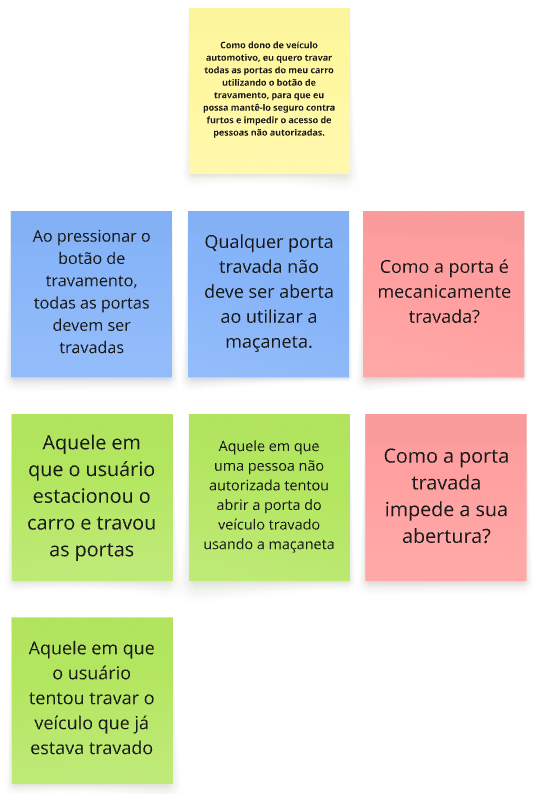
\includegraphics[height=12cm]{figuras/user_story_1.png}
\caption{História de Usuário 1: Travamento de todas as portas.}
\label{fig:historia1}
\end{figure}

Antes de seguir para a próxima história de usuário, aqui serão tratadas as perguntas que foram anotadas nesta seção. Esta etapa poderia ser postergada 
para o final do processo de discussão de exemplos, mas para garantir uma evolução incremental do produto, a próxima história será tratada quando os pontos 
abertos da atual forem respondidos.

Assim como descrito por \cite{reif2017locking}, sabe-se que existem 2 principais tipos de sistemas de travamento de porta que podem ser encontrados em veículos modernos:
\begin{itemize}
    \item Trava mecânica que é operada de maneira elétrica ou pneumática;
    \item Trava eletrônica que é montada com a trava e os eletrônicos embutidos.
\end{itemize}

Neste projeto, será implementado uma versão simulada de um sistema de trava eletrônica para se aproveitar de sua simplificação e menor número de componentes 
mecânicos no produto físico. Tipicamente, nesse sistema as maçanetas não precisam se mover ou podem até serem removidas inteiramente, podendo ser substituídas 
por botões equipados com sensores que se comunicam com a trava. Além disso, todos os componentes que transmitem o movimento da maçaneta no sistema mecânico aqui 
são desnecessários, substituídos pela fiação que se liga ao componente.

Embutido na trava eletrônica também é incluído o mecanismo básico de travamento como descrito por \cite{reif2017locking}. Ele é composto por três peças principais: 
o trinco (1) e engate (2) — que são acoplados à porta — e  o pino de batente (3) — que é acoplado ao chassi do veículo. Eles são responsáveis por manter a porta 
firmemente fechada, conforme ilustrado na figura 2:

\begin{figure}[H]
\centering
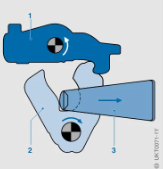
\includegraphics[height=6cm]{figuras/trava_mecanismo.png}
\caption{Mecanismo de travamento da porta \cite{reif2017locking}.}
\label{fig:travaporta}
\end{figure}

Durante o fechamento da porta, o engate (2) colide com o pino de batente (3) e gira no sentido anti-horário, passando por baixo do pino até retornar à sua posição 
inicial e fazer contato com o trinco (1). Nesse ponto, a trava encontra-se na posição fechada, exatamente como demonstrado na imagem, e qualquer tentativa de abrir 
a porta força o engate no sentido horário — movimento que é impedido pela presença do trinco.

Quando a porta está destravada, no entanto, é possível abri-la ao girar o trinco no sentido anti-horário. Esse movimento libera o engate, permitindo que ele se 
afaste do pino de batente e possibilite a abertura da porta.

No caso da trava eletrônica, o acionamento desse mecanismo é controlado por lógica implementada em software e transmitido por meio de um motor que é mecanicamente 
conectado ao trinco. Assim, respondendo à segunda pergunta, a porta trava se mantém fechada ao bloquear o movimento do trinco mediante o uso da maçaneta, da mesma 
forma que a abertura é feita ao mover o trinco.

Para modelar esse comportamento do sistema, o seu escopo pode ser definido em termos de lógica de aplicação e de software básico da seguinte maneira:

\begin{itemize}
    \item \textbf{Lógica de aplicação} - gera saídas em binário para cada porta, definindo se ela está travada ou destravada e se ela deve ser aberta ou mantida fechada;
    \item \textbf{Lógica de software básico} - recebe o sinal de saída em 0 ou 1 e o converte em sinais compreensíveis para o hardware de travamento, que resultam no movimento do motor.
\end{itemize}

Além do mecanismo de travamento em si, serão utilizados botões para realizar o travamento e abertura das portas. Seu escopo será feito de maneira similar, utilizando 
valores binários como abstrações dos sinais existentes a nível de hardware que são convertidos no software básico. Em suma, para atender a primeira história de 
usuário discutida, o modelo do sistema será desenvolvido tomando como base a lógica de aplicação assim como destacado na figura 3:

\begin{figure}[H]
\centering
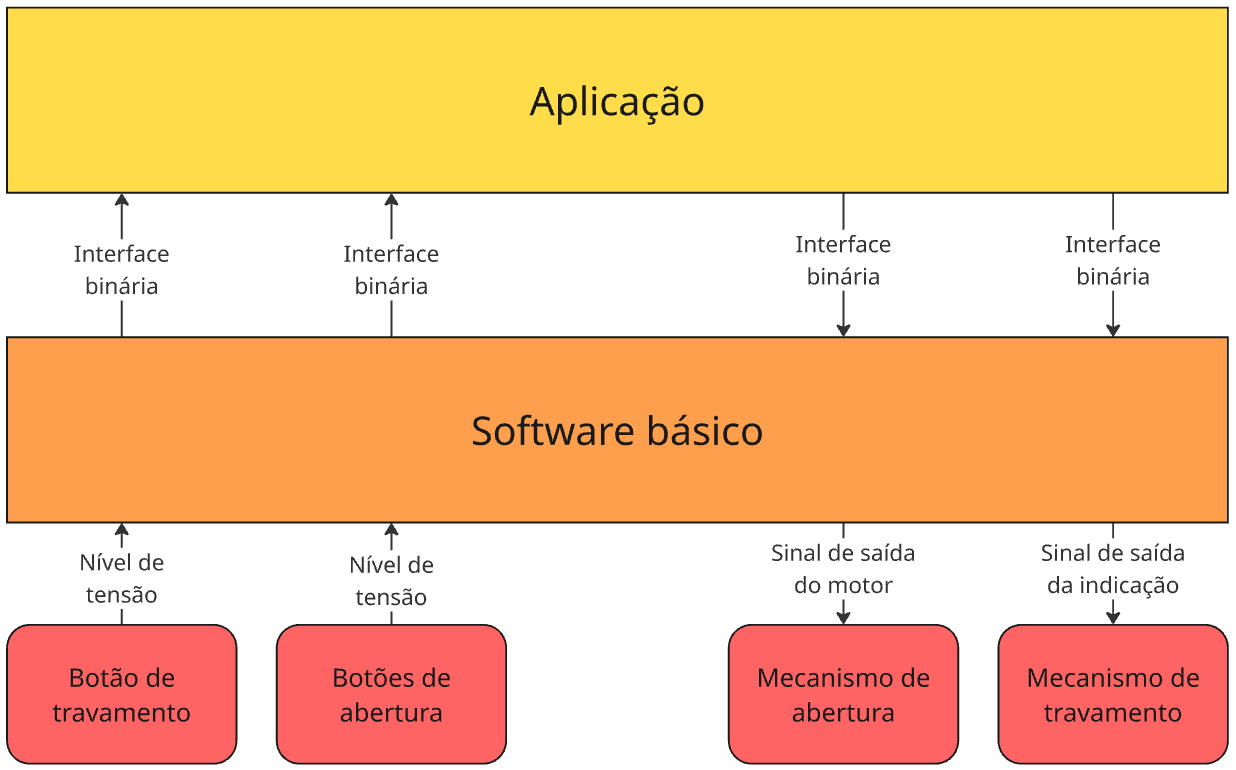
\includegraphics[height=8cm]{figuras/diagrama_aplication.png}
\caption{Diagrama de abstração do sistema em camadas de aplicação, software básico e componentes físicos.}
\label{fig:abstracaosw}
\end{figure}

Portanto, para a lógica de aplicação do modelo, receber o valor 1 recebido pela interface binária do botão de travamento é interpretado como um comando de 
pressionamento, da mesma forma que o valor 1 na interface do botão de abertura indica que a maçaneta foi acionada. No sentido oposto, ao enviar a saída para 
o software básico, esses valores são interpretados e convertidos em sinais de controle que determinam o movimento do motor.

Na prática, o travamento ou destravamento funciona apenas como uma limitação à abertura das portas e portanto, especialmente no caso da trava eletrônica, 
não há distinção física evidente entre os dois estados. Para facilitar essa identificação, este trabalho introduz uma indicação adicional, representada 
pelo "Mecanismo de travamento" na figura \ref{fig:abstracaosw}. Ela servirá apenas para indicar o estado atual de cada porta, facilitando a execução dos testes e a validação 
funcional do sistema.

\subsection{História de usuário 2}
\label{sbs:historia2}

Ao considerar a história de usuário de destravamento das portas, é importante pensar na perspectiva da intenção de acessar o veículo. Isso é uma situação 
cotidiana que acontece com altíssima frequência, e portanto possui exemplos muito semelhantes a história 1:

\begin{itemize}
    \item \textbf{Aquele em que o usuário destravou as portas e entrou no carro} — situação típica de uso, ocorre sempre que o usuário retorna ao carro e precisa acessá-lo normalmente após o destravamento;
    \item \textbf{Aquele em que algumas portas já estavam destravadas} - caso em que o veículo se encontrava parcial ou totalmente destravado no momento em que o botão de destravamento foi acionado;
    \item \textbf{Aquele em que o usuário abriu a porta que estava destravada} —  situação em que, após o destravamento, o usuário acessa o veículo por meio da maçaneta, uma vez que a porta está destravada.
\end{itemize}

Para satisfazer os exemplos listados, as seguintes regras serão implementadas:

\begin{itemize}
    \item Ao pressionar o botão de destravamento, todas as portas devem ser destravadas.
    \item Qualquer porta destravada deve ser aberta ao utilizar a maçaneta.
\end{itemize}

Ao final, foram capturados 3 exemplos e 2 regras na história de usuário, o que compõe as seguintes notas coloridas:

\begin{figure}[H]
\centering
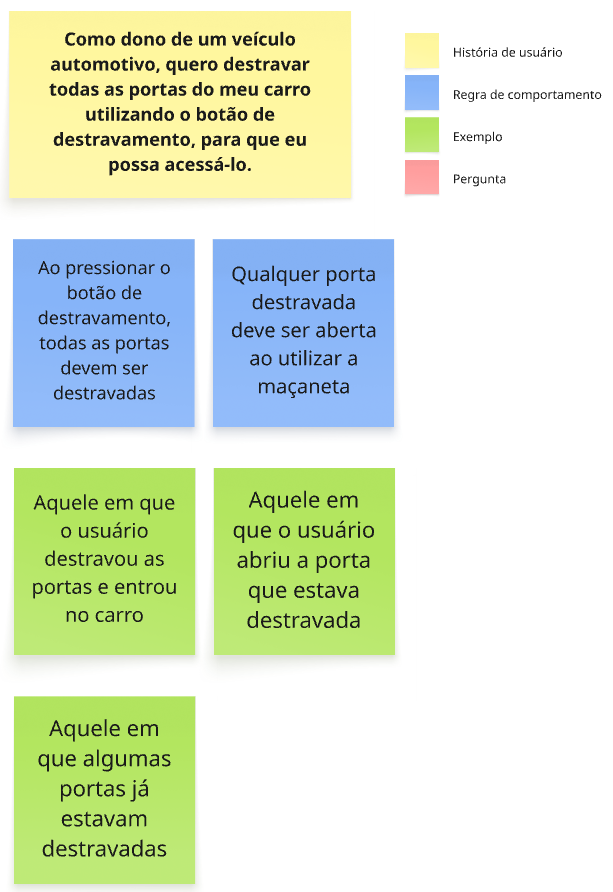
\includegraphics[height=12cm]{figuras/user_story_2.png}
\caption{História de Usuário 2: Destravamento de todas as portas.}
\label{fig:historia2}
\end{figure}

Com base nas respostas obtidas na história anterior, diversas incertezas acerca do funcionamento do destravamento das portas já foram determinadas. Sabe-se, 
por exemplo, que a porta destravada possui uma indicação de estado e que, ao pressionar o botão de abertura, a saída do modelo deve informar ao software básico 
que o mecanismo da porta deve ser liberado — ação que será realizada por meio do sinal de controle enviado ao motor.

A única distinção nesta história é a introdução de um novo botão: o botão de destravamento. Ele exige uma interface semelhante à descrita anteriormente, sendo 
igualmente interpretada pelo software básico como um valor de tensão e convertido em um sinal binário que indica o estado atual do botão.

\subsection{História de usuário 3}

A indicação da confirmação de travamento ou destravamento do veículo tem a grande importância de permitir que o usuário esteja assegurado de que o seu comando foi 
recebido e executado pelo veículo. Ela deve portanto ser invocada sempre que o usuário estiver utilizando as histórias 1 e 2, além de capturar 
os seguintes exemplos:

\begin{itemize}
    \item \textbf{Aquele em que o usuário travou seu veículo e ficou na dúvida se as portas foram travadas ou destravadas} - caso em que o usuário utiliza o botão de travamento e espera que o seu veículo seja assegurado. Deve invocar uma indicação distinta da indicação de destravamento;
    \item \textbf{Aquele em que o usuário destravou seu veículo e ficou na dúvida se as portas foram travadas ou destravadas} - caso em que o usuário utiliza o botão de destravamento e espera que o seu veículo seja destravado. Deve invocar uma indicação distinta da indicação de travamento;
    \item \textbf{Aquele em que o usuário tentou travar seu veículo sem perceber que uma das portas ficou aberta} - pode acontecer quando uma ou mais portas ficam abertas por conta de alguém esquecer de fechá-la. Neste caso, mesmo travando a porta que está aberta, o veículo ainda não fica seguro contra o acesso indevido e portanto deve invocar uma indicação de falha.
\end{itemize} 

As regras que cobrem os exemplos listados são:

\begin{itemize}
    \item O veículo deve indicar que foi travado ou destravado com sucesso utilizando sinais distintos para cada comando;
    \item O veículo deve indicar com um sinal de falha quando pelo menos uma das portas está aberta ao receber o comando de travamento.
\end{itemize}

O último exemplo levanta questões que precisam ser exploradas por meio de perguntas e trazem consigo um novo fator que o sistema deve considerar: o estado de 
abertura das portas. Para isso, as seguintes perguntas são criadas:

\begin{itemize}
    \item Como o sistema detecta se uma porta está aberta ou fechada?
    \item É possível travar ou destravar uma porta que está aberta?
\end{itemize}

Dessa forma, essa história de usuário foi mapeada com 3 exemplos, 2 regras e 2 perguntas, de acordo com a figura \ref{fig:historia3}:

\begin{figure}[H]
\centering
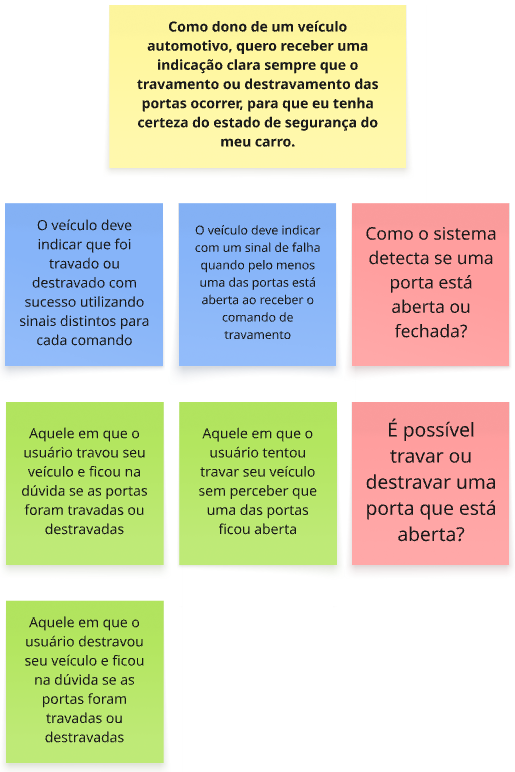
\includegraphics[height=12cm]{figuras/user_story_3.png}
\caption{História de Usuário 3: Feedback de travamento.}
\label{fig:historia3}
\end{figure}

A investigação das perguntas levantadas envolvem detalhes que dependem diretamente da implementação física do produto. Para respondê-las, é necessário 
compreender como um sistema veicular real consegue identificar se as portas estão fisicamente abertas.

Esta detecção é normalmente feita por meio de sensores ou mecanismos capazes de indicar quando a porta está entreaberta (estado \textit{ajar}). Um exemplo é 
apresentado em \citeonline{us4566285a}, que descreve o uso de switches físicos: eles são pressionados quando a porta está completamente fechada e liberados 
quando a porta se abre. 

Esse tipo de sensor pode ser integrado de forma semelhante às interfaces binárias utilizadas nos botões de travamento e destravamento, empregando sinais 
binários (0 ou 1) para representar os estados "fechada" ou "aberta" da porta. Com essa informação, o sistema pode combinar o estado físico da porta com a 
entrada da interface do botão de travamento para determinar quando o alerta para o usuário deve ser realizado.

É importante destacar que, embora o controle de abertura da porta seja gerenciado pelo sistema, a utilização de um sensor continua sendo essencial para 
determinar seu estado real. Esse cenário é comum no controle de componentes mecânicos, em que parte do comportamento não é governada diretamente pela 
lógica de software ou eletrônica.

No caso em questão, a saída final do sistema de travamento consiste no acionamento do motor que movimenta o trinco e libera o mecanismo da trava, permitindo 
que a porta seja aberta. No entanto, uma vez que essa ação é executada, o sistema não tem como saber se o usuário realmente abriu a porta — ou se, após abri-la, 
voltou a fechá-la — sem o auxílio de um sensor. Isso ocorre porque a abertura da porta é uma ação mecânica realizada pelo usuário, sendo apenas condicionada, e 
não diretamente executada, pelo sistema eletrônico em desenvolvimento.

Além disso, o travamento e destravamento das portas é realizado de maneira independente do estado da porta e pode ser realizado mesmo que ela esteja aberta. Isso 
deve-se ao fato de que o controlador eletrônico é responsável por definir quando o mecanismo da trava deve ser acionado. Caso a porta esteja destravada, esta ação 
é tomada após o pressionar do botão de abertura da porta.

Em termos práticos, isso significa que não existe diferença física entre uma porta travada ou destravada, este é apenas um estado que é virtualmente definido 
pelo controlador. É importante ressaltar que travar uma porta aberta ainda não satisfaz a condição de assegurar o veículo, como definido na primeira história 
de usuário e por conta disso o alerta do usuário se vê necessário.

\subsection{História de usuário 4}

A funcionalidade de \textit{Keyless Access} permite o destravamento individual das portas assim que o usuário aciona a maçaneta de uma porta travada, desde que a chave 
autorizada esteja presente em sua posse. Os exemplos de uso dessa funcionalidade são bastante semelhantes aos do destravamento convencional, pois refletem 
situações em que o usuário tem a intenção de acessar o veículo. 

Neste estágio, ainda não foi definida a tecnologia que será utilizada para a identificação da chave. Por isso, essa incerteza será tratada por meio de uma 
pergunta associada a esta história de usuário.

Os exemplos capturados na discussão da história são:

\begin{itemize}
    \item \textbf{Aquele em que o usuário tinha a chave no bolso e usou a maçaneta} — Este é o caso típico de uso da funcionalidade: a chave autorizada está próxima e é reconhecida pelo sistema, permitindo o destravamento imediato da porta acionada;
    \item \textbf{Aquele em que outra pessoa abriu outra porta simultaneamente} — Neste caso, mais uma porta é aberta simultaneamente, possivelmente por alguém acompanhando o dono do veículo. O sistema deve tratar as portas de forma independente, e portanto ambas devem ser destravadas individualmente, permitindo o acesso simultâneo;
    \item \textbf{Aquele em que o usuário destravou a porta e a fechou de novo} — Após acessar o veículo utilizando o \textit{Keyless Access} e em seguida fechar a porta, o sistema deve manter a porta destravada até que o usuário execute explicitamente o comando de travamento. Isso garante que a intenção do usuário seja respeitada e evita travamentos não intencionais.
\end{itemize}

Para cobrir os exemplos, as seguintes regras serão utilizadas:

\begin{itemize}
    \item Qualquer porta que tiver sua maçaneta utilizada deve ser destravada desde que a chave esteja próxima ao veículo;
    \item A porta deve ser mantida destravada após a operação de \textit{Keyless Access}.
\end{itemize}

O mapeamento de exemplos dessa história na forma de notas coloridas é composto por 3 exemplos, 2 regras e 1 pergunta:

\begin{figure}[H]
\centering
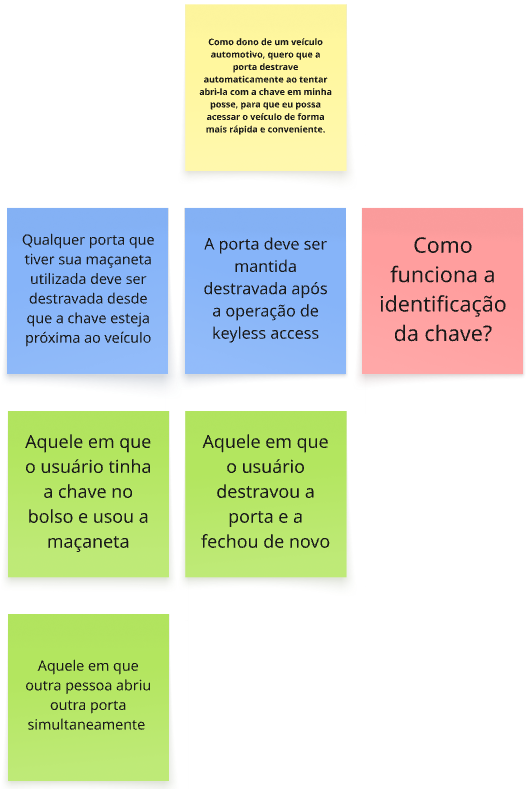
\includegraphics[height=12cm]{figuras/user_story_4.png}
\caption{História de Usuário 4: \textit{Keyless Access}.}
\label{fig:historia4}
\end{figure}

Por fim, uma nova pergunta foi levantada no mapeamento de exemplos da história e deve ser respondida antes do trabalho na próxima história. Para fazê-lo, é 
preciso investigar alguma opção de tecnologia que possa ser utilizada para representar a validação de chave de usuário. 

A implementação de sistemas de detecção de chave, conforme descrito por \citeonline{glocker2016protocol}, costumam utilizar módulos de comunicação por rádio-frequência (RF), 
capazes de estabelecer conexão com um dispositivo autorizado. A validação desse dispositivo pode ser realizada por meio de diferentes métodos e protocolos de segurança, 
que incluem mecanismos de autenticação mútua entre a chave e o veículo. Esses protocolos aumentam a robustez do sistema contra tentativas de acesso não autorizado.

Em casos mais simples, como demonstrado em \citeonline{arduinoRFID}, o sistema utiliza um sensor \textit{RFID (Radio Frequency Identification)} e uma tag que contém uma chave 
de identificação única. O funcionamento baseia-se na transmissão do identificador por meio de um sinal de rádio quando a tag é aproximada do sensor. O sensor, 
por sua vez, envia o código recebido ao microcontrolador, que o compara com um identificador previamente armazenado em sua memória. Caso haja correspondência, 
a chave é considerada válida e o acesso é autorizado.

Esse tipo de autenticação, no contexto da arquitetura \textit{AUTOSAR}, é normalmente responsabilidade de um componente específico do software básico pertencente 
à pilha de cibersegurança. Esse componente, conhecido como \textit{Key Manager} \cite{autosarKeyManager}, fornece serviços utilizados para a validação de chaves, 
utilizando diferentes protocolos de segurança. Ele também se comunica com a unidade de memória do controlador para acessar os dados das chaves previamente registradas.

Considerando a presença desse componente no sistema \textit{AUTOSAR}, será adotada novamente uma abstração da tecnologia de hardware envolvida, por meio de uma interface 
binária. Nesse cenário, a verificação da chave de identificação em relação ao valor armazenado em memória é realizada pelo \textit{Key Manager} e o resultado dessa 
validação é então comunicado à aplicação de forma semelhante ao funcionamento dos botões de entrada: por meio de um sinal binário que indica se a chave foi 
validada (1) ou não (0).

\subsection{História de usuário 5}
A funcionalidade de auto travamento é comumente implementada para contemplar diferentes cenários de uso do veículo. Neste caso específico, o foco está na situação em 
que as portas são destravadas de forma não intencional. Antes de apresentar os exemplos, será feita uma definição do que se entende por "não intenção" por parte do 
usuário, considerando que, na prática, essa intenção precisa ser inferida com base nas entradas disponíveis no sistema. 

Esse tipo de questão costuma ser capturado em perguntas, nas notas vermelhas, para que possa ser investigado após o mapeamento de exemplos. No entanto, para essa 
história é essencial que a definição de não intencional seja feita, pois ela definirá com clareza que exemplos de uso devem ser mapeados.

De modo geral, o destravamento das portas tem como objetivo permitir o acesso ao veículo, o que se concretiza quando o usuário abre pelo menos uma das portas. Utilizando 
esse critério, a ausência da abertura das portas dentro de um determinado intervalo de tempo após o destravamento pode ser interpretada como um indicativo de que o 
usuário não teve a intenção consciente de destravar o veículo. 

Essa condição também é presente em veículos Volkswagen, assim como descrito no manual do usuário \cite{vwLocking}. Segundo ele, o veículo realiza o travamento automático 
em até 45 segundos após ter sido destravado, desde que, entre outras possíveis condições, nenhuma das portas tenha sido aberta. A fim de tornar a ação de travamento 
automático mais rápida e facilitar a execução dos testes, o tempo de espera para essa condição será reduzido para 15 segundos neste trabalho.

Adicionalmente, o estado inicial das portas no momento do destravamento também é de relevância para esse comportamento. Nos casos em que o veículo não estava 
completamente travado previamente, infere-se que o usuário não possuía a intenção de garantir a segurança do veículo, mesmo antes do botão de destravamento ser 
pressionado, e portanto ele não precisa ser travado novamente.

Sabe-se que o principal objetivo do travamento do veículo é garantir sua segurança contra furtos e impedir o acesso de pessoas não autorizadas. No entanto, existem 
cenários em que o usuário pode intencionalmente optar por deixar o veículo destravado, mesmo que não pretenda acessá-lo de imediato. Um exemplo disso seria quando 
o veículo é deixado em uma garagem particular, onde o usuário deseja mantê-lo acessível para buscar um item posteriormente ou por qualquer outro motivo, sem a 
necessidade de utilizar novamente a chave ou o sistema de \textit{Keyless Access}.

Para contemplar essa situação e permitir que a intenção do usuário seja respeitada, é necessário que exista pelo menos uma regra específica que permita o 
destravamento completo, sem que seja necessário o acesso ao veículo. Neste caso, será adotada a estratégia de considerar o duplo acionamento do botão de 
destravamento como uma indicação explícita da intenção de manter o veículo destravado.

Por fim, os exemplos capturados na história são:

\begin{itemize}
    \item \textbf{Aquele em que o usuário destravou mas não foi acessar o carro} — este é o cenário padrão de destravamento não intencional, que pode ocorrer por diversos motivos, como o acionamento acidental do botão de destravamento. Nessa situação, o sistema realizará o travamento automático após um intervalo de tempo pré-definido, interpretando que não houve intenção de acesso;
    \item \textbf{Aquele em que o usuário destravou e foi acessar o carro} — neste cenário, a situação oposta à do exemplo anterior acontece, pois o usuário acessou o veículo, abrindo uma das portas, em tempo. O travamento automático não deve ser acionado neste caso;
    \item \textbf{Aquele em que o usuário pressionou o botão de destravamento duas vezes para manter o carro destravado sem precisar abrir uma porta} — Quando for da intenção do usuário deixar o veículo destravado sem abrir nenhuma porta, a função de travamento automático será inibida mediante o duplo acionamento do botão de destravamento. Essa ação será interpretada como uma indicação explícita da intenção de manter o veículo acessível;
    \item \textbf{Aquele em que o usuário destravou o veículo quando ele já estava acessível} — refere-se às situações em que o veículo não estava completamente travado inicialmente, seja porque uma ou mais portas já estavam destravadas ou por conta do acionamento repetido do botão de destravamento. Nestes casos, o sistema entende que o usuário já interagiu com o veículo e portanto o travamento automático também não será executado.
\end{itemize}

Com os exemplos mapeados, o comportamento definido garante que o travamento automático trata em específico os casos em que a ação do usuário indicou que ele não possuía a intenção de mudar o veículo de um estado inicial em que ele está absolutamente seguro contra furtos - todas as portas estavam travadas - para o caso em que qualquer pessoa poderia acessá-lo. As regras que satisfazem os exemplos são:

\begin{itemize}
    \item Travar automaticamente caso o botão de destravamento seja usado uma vez e nenhuma porta seja aberta;
    \item Não travar caso o botão de destravamento seja pressionado uma segunda vez;
    \item Não travar caso o veículo não esteja completamente travado antes do destravamento.
\end{itemize}

O mapeamento de exemplos dessa história na forma de notas coloridas é composto por 4 exemplos e 3 regras:

\begin{figure}[H]
\centering
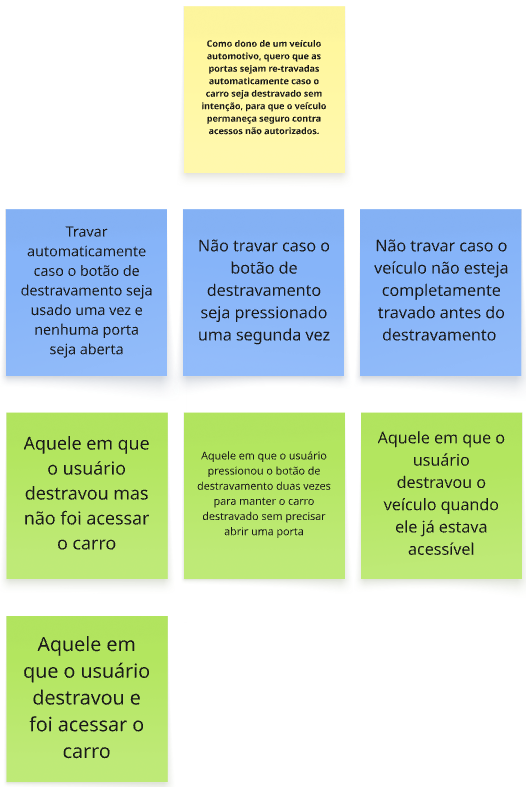
\includegraphics[height=12cm]{figuras/user_story_5.png}
\caption{História de Usuário 5: Travamento automático.}
\label{fig:historia5}
\end{figure}

\section{\textbf{Etapa 3: Desenho do diagrama de caixa preta}}
Com todas as histórias de usuário definidas, o próximo passo do trabalho consiste na elaboração do diagrama de caixa preta, com o objetivo de identificar todas as 
interfaces necessárias para suportar os comportamentos previamente levantados. Essa etapa é essencial para garantir que todas as interações entre o usuário e o 
sistema estejam claramente especificadas e para suportar a criação dos cenários \textit{Gherkin} a seguir.

Para dar início ao processo, é necessário listar todas as entradas e saídas do sistema:

\textbf{Entradas}:

\begin{itemize}
    \item Botão de travamento
    \item Botão de destravamento
    \item Botões de abertura das portas (4 no total)
    \item Sensores de abertura das portas (4 no total)
    \item Detecção de chave autenticada.
\end{itemize}

\textbf{Saídas}:

\begin{itemize}
    \item Indicação de estado de travamento de todas as portas (4 no total)
    \item Estado da tranca de cada porta (4 no total)
    \item Feedback para o usuário.
\end{itemize}

O diagrama é então elaborado com um bloco central representando o sistema, ao qual estão conectadas todas as interfaces previamente listadas. Neste estágio, 
o bloco central permanece sem conteúdo interno, uma vez que o objetivo é abstrair os detalhes da implementação e focar exclusivamente na definição das 
interações entre o sistema e o usuário.

Dessa forma, o diagrama assume a configuração ilustrada na figura \ref{fig:caixapreta}:

\begin{figure}[H]
\centering
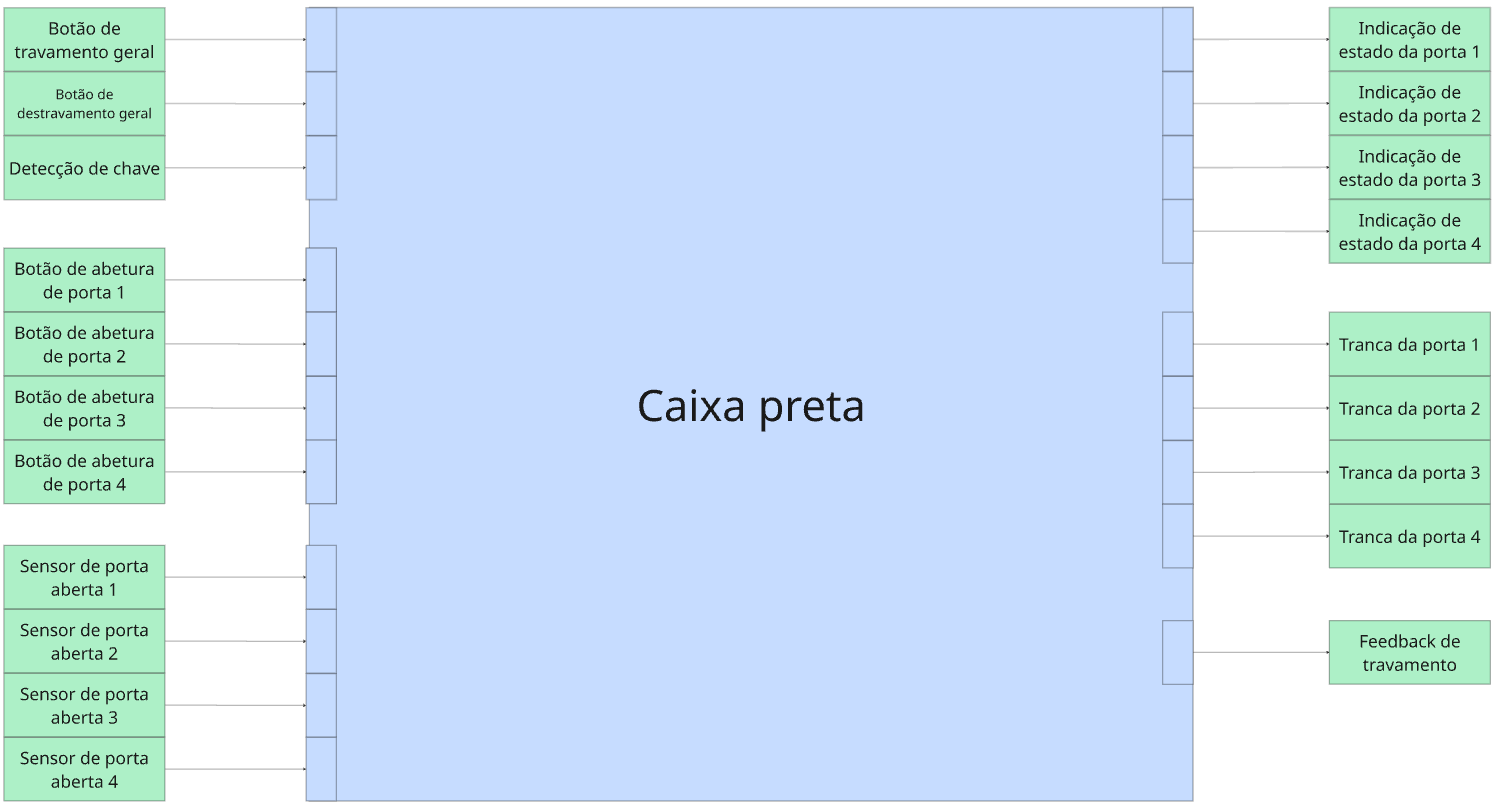
\includegraphics[height=8cm]{figuras/diagrama_caixa_preta.png}
\caption{Diagrama de Caixa Preta do sistema de travamento de portas.}
\label{fig:caixapreta}
\end{figure}

De maneira análoga, o modelo desenvolvido no Simulink também deverá adotar uma estrutura semelhante, composta por um modelo de alto nível — que define apenas as 
entradas e saídas do sistema — e um modelo de baixo nível, responsável por conter toda a lógica funcional implementada.

É importante destacar que algumas interfaces adicionais serão necessárias no modelo do sistema, embora não estejam representadas no diagrama de caixa preta, 
pois não estão diretamente relacionadas aos comportamentos observáveis pelo usuário. Essas interfaces serão detalhadas em \ref{ch:RD}, e são fundamentais para suportar aspectos técnicos que garantem o funcionamento correto do sistema. Um exemplo dessas interfaces é o tempo 
de simulação, necessário para validar a condição de auto travamento descrita na história de usuário 5.

Para finalizar essa etapa, é necessário definir quais são os valores possíveis que devem ser capturados em cada uma das interfaces criadas no diagrama da figura \ref{fig:caixapreta}.

% \begin{tabular}{|p{5cm}|p{7cm}|}
% %\centering
% %\caption{Valores possíveis para as interfaces de entrada e saída}
% %\addcontentsline{loq}{table}{\protect\numberline{\thetable}Valores possíveis para as interfaces de entrada e saída}
% \hline
% Nome da interface 1 & Valores Possíveis \\ 
% \hline
% Botão de travamento geral & 
% \begin{itemize}[topsep=0pt, partopsep=0pt, leftmargin=*]
%     \item Pressionado
%     \item Solto
% \end{itemize} \\
% \hline
% Botão de destravamento geral &
% \begin{itemize}[topsep=0pt, partopsep=0pt, leftmargin=*]
%     \item Pressionado
%     \item Solto
% \end{itemize} \\
% \hline
% Detecção de chave &
% \begin{itemize}[topsep=0pt, partopsep=0pt, leftmargin=*]
%     \item Presente
%     \item Não presente
% \end{itemize} \\
% \hline
% Botão de abetura de porta (de 1 a 4) &
% \begin{itemize}[topsep=0pt, partopsep=0pt, leftmargin=*]
%     \item Pressionado
%     \item Solto
% \end{itemize} \\
% \hline
% Sensor de porta aberta (de 1 a 4) &
% \begin{itemize}[topsep=0pt, partopsep=0pt, leftmargin=*]
%     \item Fechada
%     \item Aberta
% \end{itemize} \\
% \hline
% Indicação de estado da porta (de 1 a 4) &
% \begin{itemize}[topsep=0pt, partopsep=0pt, leftmargin=*]
%     \item Travada
%     \item Destravada
% \end{itemize} \\
% \hline
% Tranca da porta 1 &
% \begin{itemize}[topsep=0pt, partopsep=0pt, leftmargin=*]
%     \item Segura
%     \item Solta
% \end{itemize} \\
% \hline
% Feedback de travamento &
% \begin{itemize}[topsep=0pt, partopsep=0pt, leftmargin=*]
%     \item Confirmação de trava
%     \item Confirmação de destrava
%     \item Operação falha
% \end{itemize} \\
% \hline
% %\label{qua:interfaces}
% \end{tabular}

\begin{quadro}[h]
\caption{Valores possíveis para as interfaces de entrada e saída}
\label{qua:interfaces}
\begin{tabular}{|p{5cm}|p{7cm}|}
\hline
Nome da interface 1 & Valores Possíveis \\ 
\hline
Botão de travamento geral & 
\begin{itemize}[topsep=0pt, partopsep=0pt, leftmargin=*]
    \item Pressionado
    \item Solto
\end{itemize} \\
\hline
Botão de destravamento geral &
\begin{itemize}[topsep=0pt, partopsep=0pt, leftmargin=*]
    \item Pressionado
    \item Solto
\end{itemize} \\
\hline
Detecção de chave &
\begin{itemize}[topsep=0pt, partopsep=0pt, leftmargin=*]
    \item Presente
    \item Não presente
\end{itemize} \\
\hline
Botão de abertura de porta (de 1 a 4) &
\begin{itemize}[topsep=0pt, partopsep=0pt, leftmargin=*]
    \item Pressionado
    \item Solto
\end{itemize} \\
\hline
Sensor de porta aberta (de 1 a 4) &
\begin{itemize}[topsep=0pt, partopsep=0pt, leftmargin=*]
    \item Fechada
    \item Aberta
\end{itemize} \\
\hline
Indicação de estado da porta (de 1 a 4) &
\begin{itemize}[topsep=0pt, partopsep=0pt, leftmargin=*]
    \item Travada
    \item Destravada
\end{itemize} \\
\hline
Tranca da porta 1 &
\begin{itemize}[topsep=0pt, partopsep=0pt, leftmargin=*]
    \item Segura
    \item Solta
\end{itemize} \\
\hline
Feedback de travamento &
\begin{itemize}[topsep=0pt, partopsep=0pt, leftmargin=*]
    \item Sem status
    \item Confirmação de trava
    \item Confirmação de destrava
    \item Operação falha
\end{itemize} \\
\hline
\end{tabular}
\end{quadro}

Nesta tabela, os valores das interfaces foram descritos de maneira textual, com valores que se aplicam à linguagem natural proposta pela metodologia de BDD. 
Na prática, todos os valores serão utilizados como enumerações convertidas para um valor numérico que representa o estado da interface.

\section{\textbf{Etapa 4: Desenvolvimento dos cenários Gherkin}}

Nesta etapa, os cenários \textit{Gherkin} serão desenvolvidos e utilizados como critérios de aceitação das histórias previamente definidas. Estes cenários devem ser capazes 
de cobrir todos os exemplos capturados durante o mapeamento, assegurando que o desenvolvimento do sistema atenda à experiência de usuário desejada.
Como primeiro passo, será definida a estrutura de pastas do projeto, responsável por organizar tanto os arquivos \texttt{.feature} — um para cada história de usuário — 
quanto o modelo em Simulink. Seguindo a estrutura recomendada na documentação da biblioteca Behave \cite{behaveDocs}, o projeto será organizado da seguinte forma:

\begin{verbatim}
    projeto/
    |-- features/
    |   |-- lock\_all.feature
    |   |-- unlock\_all.feature
    |   |-- locking\_feedback.feature
    |   |-- unlock\_individual.feature
    |   |-- auto\_relock.feature
    |   `-- steps/
    |       `-- lock\_unlock.py
\end{verbatim}

Cada história de usuário possui um arquivo \texttt{\.feature} correspondente, todos organizados dentro da pasta \texttt{features} do projeto. A nomenclatura desses 
arquivos foi definida de forma a evidenciar a funcionalidade representada em cada um, facilitando a identificação e o rastreamento das histórias implementadas. 
Por exemplo, o arquivo \texttt{lock\_all.feature} refere-se à primeira história de usuário, que descreve a funcionalidade de travamento de todas as portas 
por meio do botão de travamento.

Além disso, o arquivo environment.py é utilizado para definir funções de inicialização que são executadas antes do início dos testes ou de cada passo individual. 
Uma de suas responsabilidades é iniciar a simulação quando os testes são acionados, além de disponibilizar interfaces que permitem a comunicação com o modelo Simulink.

Por fim, o arquivo de definição dos passos \textit{(step definitions)} é armazenado na pasta steps e foi nomeado de \texttt{lock\_unlock.py}. Ele é responsável por mapear os 
passos descritos nos cenários \textit{Gherkin} para funções executáveis, que realizam as ações esperadas e interagem com o modelo.

É importante destacar que o desenvolvimento dos cenários \textit{Gherkin} é um processo iterativo, que deve evoluir de acordo com o grau de maturidade do sistema. 
Por esse motivo, como será demonstrado na etapa de modelagem, ajustes pontuais nos cenários — como a adição de passos que facilitem a execução da simulação — 
poderão ser realizados ao longo do tempo.

Durante a criação dos cenários, alguns cuidados serão adotados para garantir consistência e reutilização. Um desses cuidados é a definição de passos genéricos 
e reutilizáveis, especialmente para ações recorrentes. Por exemplo, nas histórias 1 e 5, que descrevem funcionalidades que resultam no travamento completo do 
veículo, é possível validar o estado final utilizando um mesmo passo compartilhado, como \texttt{Then todas as portas deveriam estar travadas}.

Uma possível definição para esse passo consiste em realizar a leitura dos valores presentes nas quatro interfaces de saída do modelo, que indicam o estado atual 
de cada porta. Considerando que o valor 1 representa uma porta travada, a função deve verificar se todas as saídas possuem esse valor, aprovando o teste apenas se 
essa condição for satisfeita.

Para torná-la ainda mais reutilizável, essa função pode incorporar um parâmetro textual extraído diretamente do passo \textit{Gherkin}, permitindo que parte da frase do 
cenário seja utilizada como argumento. Dessa forma, a lógica de verificação pode ser adaptada dinamicamente: por exemplo, a função pode identificar se a última 
palavra do passo é “travadas” ou “destravadas” e, com base nisso, validar se os valores lidos são 1 (para travadas) ou 0 (para destravadas), aprovando o teste 
conforme o caso.

Outra funcionalidade importante empregada na escrita dos cenários é o uso de tabelas de exemplos \textit{(Examples)}, que possibilitam a execução repetida de um mesmo 
cenário com diferentes combinações de parâmetros. Essa abordagem é especialmente útil para validar comportamentos sob múltiplas condições iniciais, evitando a 
necessidade de duplicar cenários com estruturas idênticas.

Por exemplo, a primeira história de usuário define que, ao pressionar o botão de travamento, todas as portas devem ser travadas, independentemente de seu estado 
inicial. Para verificar esse comportamento, é possível parametrizar o estado de cada porta utilizando a cláusula Given combinada com a tabela de exemplos, 
como mostrado abaixo:

\begin{verbatim}
    Given a porta 1 está <estado1>
    
    Examples:
    | estado1    |
    | travada    |
    | destravada |
\end{verbatim}


Ao utilizar a sintaxe \texttt{<...>}, o Behave interpreta o conteúdo como uma variável, cujo valor será substituído com base nas linhas da tabela Examples. Cada 
linha da tabela gera um cenário independente, preservando a estrutura original, mas substituindo os parâmetros pelos respectivos valores.

Dessa forma, durante a execução, o Behave processa o cenário duas vezes. Na primeira execução, o passo é \texttt{Given a porta 1 está travada} e na segunda 
ele é \texttt{Given a porta 1 está destravada}.

Essa estrutura oferece grande flexibilidade na criação dos cenários e assegura a cobertura completa das possíveis combinações. No cenário real que será apresentado 
a seguir, existem 16 combinações possíveis, resultantes dos diferentes estados (travada ou destravada) das quatro portas.

Por fim, a funcionalidade \textit{Background} também será utilizada nos arquivos .feature para definir um estado inicial comum a todos os cenários. Essa estrutura permite 
declarar uma sequência de passos Given que serão executados automaticamente antes de cada cenário presente no arquivo. Isso evita a repetição de passos que se 
aplicam a múltiplos cenários, promovendo maior clareza e reutilização na especificação dos testes.

\subsection{História de usuário 1}

Uma maneira eficaz de estruturar o cenário \textit{Gherkin} é adotar a perspectiva do usuário e tentar descrever o comportamento esperado como uma sequência de ações, 
utilizando as cláusulas Given, When e Then. Tomando como base o primeiro exemplo da história — “aquele em que o usuário estacionou o carro e travou as portas” — 
o cenário pode ser representado da seguinte forma:

\begin{verbatim}
    Given o carro estava destravado ao ser estacionado
    When o usuário pressionou o botão de travamento
    Then todas as portas foram travadas
\end{verbatim}

Além disso, é possível aplicar o recurso de tabelas de exemplos \textit{(Examples)} para generalizar o cenário e incluir o segundo exemplo descrito na história: “aquele 
em que o usuário tentou travar o veículo que já estava travado”. Nesse caso, substitui-se a primeira condição \textit{(Given)} por um conjunto de passos que definem 
individualmente o estado inicial de cada porta, utilizando os valores fornecidos pela tabela para simular todas as combinações possíveis de estados iniciais. 
A resposta final do sistema é comum entre os exemplos já que ambos compartilham o mesmo resultado final — a mesma cláusula \textit{Then}. 

Dessa forma, o primeiro exemplo é coberto em uma das linhas da tabela — a que define que todas as portas estão inicialmente destravadas — e o segundo é coberto 
por todas as demais linhas — que definem todas as possíveis combinações de estado para cada porta. O cenário geral pode assumir a seguinte forma:

\begin{verbatim}
Scenario Outline: Locking all doors
    Given the door '1' is <door_1_state>
    And the door '2' is <door_2_state>
    And the door '3' is <door_3_state>
    And the door '4' is <door_4_state>

    When I press the vehicle 'lock' button
    Then all doors should be 'locked'

    Examples:
        | door_1_state | door_2_state | door_3_state | door_4_state |
        | unlocked     | unlocked     | unlocked     | unlocked     |
        | unlocked     | unlocked     | unlocked     | locked       |
        | unlocked     | unlocked     | locked       | unlocked     |
        | unlocked     | unlocked     | locked       | locked       |
        | unlocked     | locked       | unlocked     | unlocked     |
        | unlocked     | locked       | unlocked     | locked       |
        | unlocked     | locked       | locked       | unlocked     |
        | unlocked     | locked       | locked       | locked       |
        | locked       | unlocked     | unlocked     | unlocked     |
        | locked       | unlocked     | unlocked     | locked       |
        | locked       | unlocked     | locked       | unlocked     |
        | locked       | unlocked     | locked       | locked       |
        | locked       | locked       | unlocked     | unlocked     |
        | locked       | locked       | unlocked     | locked       |
        | locked       | locked       | locked       | unlocked     |
        | locked       | locked       | locked       | locked       |
\end{verbatim}

A cláusula \textit{Given} utiliza quatro passos para definir os valores iniciais de cada porta, de forma que cada um recebe uma variável correspondente a uma coluna da 
tabela de exemplos. Essa tabela contém 16 linhas, que representam todas as combinações possíveis entre os estados "travada" e "destravada" para as quatro portas.

Na cláusula \textit{When}, é descrita a ação do usuário ao pressionar o botão de travamento. Em seguida, a cláusula \textit{Then} especifica que todas as portas devem estar travadas, 
validando assim o comportamento esperado de assegurar o veículo independentemente de seu estado inicial.

O último exemplo a ser coberto é: “aquele em que uma pessoa não autorizada tentou abrir a porta do veículo travado usando a maçaneta”. Ele é validado por um 
cenário em que a porta continua fechada após a o botão de abertura ser pressionado, tendo em vista que ela está travada.

Para evitar a duplicação de cenários, a tabela de exemplos é novamente utilizada, permitindo a execução automática do teste para cada porta individualmente, variando 
apenas o ponto de interação. Ao final, o cenário assume a seguinte forma:

\begin{verbatim}

    Scenario Outline: Door cannot be released when locked
        Given the door <door_id> is 'locked'
        When I 'press' the door <door_id> release button
        Then the door <door_id> should be 'held'

        Examples:
            | door_id |
            | 1       |
            | 2       |
            | 3       |
            | 4       |

\end{verbatim}


\subsection{História de usuário 2}

A segunda história de usuário tem grande semelhança com a primeira e possui exemplos mapeados com casos de uso que são análogos à de travamento das portas. O 
primeiro cenário criado para esta história é:

\begin{verbatim}
Scenario Outline: Unlocking all doors    
    Given the door '1' is <door_1_state>
    And the door '2' is <door_2_state>
    And the door '3' is <door_3_state>
    And the door '4' is <door_4_state>

    When I press the vehicle 'unlock' button
    Then all doors should be 'unlocked'

    Examples:
        | door_1_state  | door_2_state  | door_3_state  | door_4_state  |
        | unlocked      | unlocked      | unlocked      | unlocked      |
        | unlocked      | unlocked      | unlocked      | locked        |
        | unlocked      | unlocked      | locked        | unlocked      |
        | unlocked      | unlocked      | locked        | locked        |
        | unlocked      | locked        | unlocked      | unlocked      |
        | unlocked      | locked        | unlocked      | locked        |
        | unlocked      | locked        | locked        | unlocked      |
        | unlocked      | locked        | locked        | locked        |
        | locked        | unlocked      | unlocked      | unlocked      |
        | locked        | unlocked      | unlocked      | locked        |
        | locked        | unlocked      | locked        | unlocked      |
        | locked        | unlocked      | locked        | locked        |
        | locked        | locked        | unlocked      | unlocked      |
        | locked        | locked        | unlocked      | locked        |
        | locked        | locked        | locked        | unlocked      |
        | locked        | locked        | locked        | locked        |
\end{verbatim}

Este cenário define que, com as pré-condições que cobrem todas as possíveis combinações de travamento e destravamento para cada porta, após o botão de destravamento 
ser pressionado, o veículo será destravado. Ele cobre os dois primeiros exemplos mapeados:
\begin{itemize}
    \item Aquele em que o usuário destravou as portas e entrou no carro;
    \item Aquele em que algumas portas já estavam destravadas.
\end{itemize}

Para o último exemplo, o seguinte cenário será utilizado:

\begin{verbatim}
    Scenario Outline: Door can be released when unlocked
        Given the door <door_id> is 'unlocked'
        When I 'press' the door <door_id> release button
        Then the door <door_id> should be 'released'

        Examples:
            | door_id |
            | 1       |
            | 2       |
            | 3       |
            | 4       |
\end{verbatim}

Este cenário, que é executado para cada uma das portas, define que a porta será aberta após o botão de abertura ser pressionado, tendo em vista que ela 
está destravada. Ele cobre o seguinte exemplo mapeado:

\begin{itemize}
    \item Aquele em que o usuário abriu a porta que estava destravada.
\end{itemize}


\subsection{História de usuário 3}

Para especificar o comportamento descrito nesta história, é necessário criar um novo tipo de passo que valide qual resposta de feedback foi acionada pelo veículo. 
Isso pode ser feito de acordo com o cenário:

\begin{verbatim}
Scenario Outline: Locking feedback when locking or unlocking the vehicle
    When I press the vehicle <operation> button

    Then all doors should be <state>
    And I should receive a <feedback> feedback

    Examples:
        | operation | state    | feedback               |
        | lock      | locked   | locking confirmation   |
        | unlock    | unlocked | unlocking confirmation |
\end{verbatim}

Esse cenário descreve que, ao pressionar o botão correspondente, todas as portas devem ser travadas ou destravadas, e um feedback específico deve ser emitido. A cláusula \textit{Given} foi omitida neste caso, pois o estado inicial do veículo — seja total ou parcialmente travado/destravado — não deve influenciar 
o resultado esperado. Ou seja, independentemente da condição inicial, o sistema deve aplicar a ação solicitada e fornecer o feedback apropriado.

Os seguintes exemplos são cobertos neste cenário:

\begin{itemize}
    \item Aquele em que o usuário travou seu veículo e ficou na dúvida se as portas foram travadas ou destravadas;
    \item Aquele em que o usuário destravou seu veículo e ficou na dúvida se as portas foram travadas ou destravadas;
\end{itemize}

O último exemplo dessa história é: “aquele em que o usuário tentou travar seu veículo sem perceber que uma das portas ficou aberta” e será coberto no seguinte cenário:

\begin{verbatim}
Scenario Outline: Failure feedback when one door is open
    Given the door <door_id> is 'unlocked'
    And the door <door_id> is <door_open_state>

    When I press the vehicle 'lock' button

    Then all doors should be 'locked'
    And I should receive a <feedback_received> feedback

    Examples:
        | door_id | door_open_state | feedback_received    |
        | 1       | open            | operation failed     |
        | 2       | open            | operation failed     |
        | 3       | open            | operation failed     |
        | 4       | open            | operation failed     |
        | 1       | closed          | locking confirmation |
        | 2       | closed          | locking confirmation |
        | 3       | closed          | locking confirmation |
        | 4       | closed          | locking confirmation |
\end{verbatim}

Este cenário estabelece como pré-condição que uma das quatro portas está destravada, podendo estar aberta ou fechada, conforme os valores definidos na tabela de exemplos. 
Com base nesse estado inicial, ao pressionar o botão de travamento, o sistema deve emitir um feedback específico: “operação falha” caso a porta esteja aberta, ou 
“confirmação de travamento” caso ela esteja fechada.

Além disso, o cenário específica que, independentemente de a porta estar aberta ou fechada, todas as portas devem ser marcadas como travadas após a ação. Isso está 
de acordo com a análise realizada durante a investigação das perguntas desta história, a qual identificou que o travamento ou destravamento de uma porta aberta é possível. 
Isso ocorre porque o conceito de “estado da porta” não está vinculado a uma ação física imediata, mas sim a um estado lógico atribuído pelo controlador que é definido 
de forma virtual no sistema.


\subsection{História de usuário 4}

Para cobrir essa história, o primeiro exemplo considerado é “aquele em que o usuário tinha a chave no bolso e usou a maçaneta”, o qual está representado pelo seguinte cenário:

\begin{verbatim}
Scenario Outline: Unlocking a single door when I have the key
    Given the door <door_id> is 'locked'
    And I have an authenticated key with me

    When I 'press' the door <door_id> release button

    Then the door <door_id> should be 'unlocked'
    And the door <door_id> should be 'released'

    Examples:
        | door_id |
        | 1       |
        | 2       |
        | 3       |
        | 4       |
\end{verbatim}

O cenário define que a porta encontra-se inicialmente travada e, ao ser pressionado o botão de abertura enquanto o usuário está em posse da chave, ela deveria 
ser destravada e aberta. A tabela de exemplos foi novamente utilizada para assegurar que esse comportamento seja testado em todas as portas.

O próximo exemplo é “aquele em que outra pessoa abriu outra porta simultaneamente”, o qual está coberto pelo seguinte cenário:

\begin{verbatim}
Scenario Outline: Unlocking multiple single doors when I have the key   
    Given all doors are 'locked'
    And I have an authenticated key with me

    When I 'press' the door <door_id_1> release button
    And I 'press' the door <door_id_2> release button

    Then the door <door_id_1> should be 'unlocked'
    And the door <door_id_1> should be 'released'
    And the door <door_id_2> should be 'unlocked'
    And the door <door_id_2> should be 'released'

    Examples:
        | door_id_1 | door_id_2 |
        | 1         | 2         |
        | 1         | 3         |
        | 1         | 4         |
        | 2         | 1         |
        | 2         | 3         |
        | 2         | 4         |
        | 3         | 1         |
        | 3         | 2         |
        | 3         | 4         |
        | 4         | 1         |
        | 4         | 2         |
        | 4         | 3         |
\end{verbatim}

A estrutura do cenário é semelhante à anterior, porém com a adição de novos passos que simulam o pressionamento do botão, o destravamento e a abertura de duas 
portas simultaneamente. Para isso, foram utilizadas variáveis distintas para cada porta, permitindo que a tabela de exemplos cubra todas as possíveis combinações 
de abertura simultânea entre duas portas.

Por fim, o último exemplo é “aquele em que o usuário destravou a porta e a fechou de novo”, que é coberto pelo cenário:

\begin{verbatim}
    Scenario Outline: Individual door is left unlocked
        Given the door <door_id> is 'locked'
        And I have an authenticated key with me

        When I 'press' the door <door_id> release button
        And I wait '1' seconds
        And I 'release' the door <door_id> release button

        Then the door <door_id> should be 'unlocked'
        And the door <door_id> should be 'held'

        Examples:
            | door_id |
            | 1       |
            | 2       |
            | 3       |
            | 4       |
\end{verbatim}

Este cenário também é executado repetidamente para cada porta, e apresenta a diferença que, após 1 segundo de espera, o botão de abertura que havia sido pressionado 
é solto. Com essa sequência de execução, a resposta do sistema é a de manter a porta destravada, mas de deixar o trinco da trava em sua posição fechada - o que equivale 
a porta estar sendo segurada.


\subsection{História de usuário 5}

Nesta história, a utilização de medidas de tempo é um elemento essencial para garantir que a resposta do sistema esteja alinhada ao comportamento esperado. Isso 
se deve à regra que determina que o auto-travamento das portas deve ocorrer 15 segundos após o destravamento, caso nenhuma porta seja aberta nesse intervalo.

O primeiro exemplo nesta história é “aquele em que o usuário destravou mas não foi acessar o carro” que é coberto pelo cenário:

\begin{verbatim}
Scenario Outline: Auto relocking
    Given all doors are <initial_state>
    And the vehicle 'unlock' button has been pressed

    When I wait <wait_time> seconds

    Then all doors should be <expected_state>

    Examples:
        | initial_state | wait_time | expected_state |
        | locked        | 5         | unlocked       |
        | locked        | 10        | unlocked       |
        | locked        | 14        | unlocked       |
        | locked        | 15        | locked         |
        | locked        | 16        | locked         |
        | unlocked      | 5         | unlocked       |
        | unlocked      | 10        | unlocked       |
        | unlocked      | 14        | unlocked       |
        | unlocked      | 15        | unlocked       |
        | unlocked      | 16        | unlocked       |
\end{verbatim}

Esse cenário descreve que, após o botão de destravamento ser pressionado, seguido da espera de um determinado valor de tempo, o estado final das 
portas deve corresponder ao valor definido na variável de saída. O auto-travamento é efetivamente acionado nas linhas 4 e 5 da tabela, que representam 
portas inicialmente travadas, seguidas por uma espera que atende ao requisito de 15 segundos ou mais. 

Os valores de tempo utilizados na tabela foram selecionados para representar situações reais e cobrir tanto casos em que a condição de tempo é satisfeita 
quanto situações de limite. Como nas linhas que utilizam 14, 15 e 16 segundos, que validam que o sistema responde corretamente em valores que são extremamente 
próximos da janela temporal especificada.

O próximo exemplo é “aquele em que o usuário destravou e foi acessar o carro”, ilustrando uma situação em que a condição para o auto-travamento não é satisfeita, 
pois uma das portas foi aberta. Esse caso é coberto no seguinte cenário:

\begin{verbatim}
Scenario Outline: Not auto relocking if release button is pressed
    Given all doors are 'locked'
    And the vehicle 'unlock' button has been pressed
    And the release button on door <door_id> is 'released'
    And the release button on door <door_id> is 'pressed'

    When I wait '15' seconds

    Then all doors should be 'unlocked'

    Examples:
        | door_id |
        | 1       |
        | 2       |
        | 3       |
        | 4       |
\end{verbatim}

Neste exemplo, não foram definidos valores de tabela para testar múltiplas variações de estado inicial do veículo ou de tempos de espera. Essa decisão se deve ao 
fato de que o próprio exemplo descreve explicitamente uma condição na qual, mesmo a espera de tempo sendo satisfeita, o auto-travamento não deve ser acionado.

A pré-condição definida no primeiro passo estabelece que todas as portas estão inicialmente travadas, o que atende ao requisito inicial para o auto-travamento. 
A diferença ocorre no momento em que, após o uso do botão de destravamento, o botão de abertura de uma das portas é pressionado. Assim, mesmo após a espera de 
15 segundos (tempo exigido para o auto-travamento), as portas devem permanecer destravadas.

O terceiro exemplo desta história é “aquele em que o usuário pressionou o botão de destravamento duas vezes para manter o carro destravado sem precisar abrir uma 
porta”, representando outra condição em que o auto-travamento não deve ser acionado. Esse caso é coberto pelo seguinte cenário:

\begin{verbatim}
    Scenario: Not auto relocking if unlock button is pressed twice
        Given all doors are 'locked'
        And the vehicle 'unlock' button has been pressed
        And the vehicle 'unlock' button has been pressed

        When I wait '15' seconds

        Then all doors should be 'unlocked'
\end{verbatim}

Assim como no cenário anterior, não foram utilizadas variáveis para representar diferentes condições iniciais, pois o próprio exemplo também estabelece uma condição 
em que o auto-travamento não deve ocorrer. A diferença aqui está na inclusão de um segundo acionamento do botão de destravamento logo no início da sequência.

Por fim, o último exemplo desta história é “aquele em que o usuário destravou o veículo quando ele já estava acessível”, descrevendo a situação em que o auto-travamento 
não deve ser acionado caso pelo menos uma das portas já esteja destravada no início. Esse caso é tratado no seguinte cenário:

\begin{verbatim}
    Scenario Outline: Not auto relocking if some doors are unlocked
    Given the door '1' is <door_1_state>
    And the door '2' is <door_2_state>
    And the door '3' is <door_3_state>
    And the door '4' is <door_4_state>
    And the vehicle 'unlock' button has been pressed
    
    When I wait '15' seconds
    
    Then all doors should be <final_state>
    
    Examples:
    | d1 | d2 | d3 | d4 | final |
    | u  | u  | u  | u  | u     |
    | u  | u  | u  | l  | u     |
    | u  | u  | l  | u  | u     |
    | u  | u  | l  | l  | u     |
    | u  | l  | u  | u  | u     |
    | u  | l  | u  | l  | u     |
    | u  | l  | l  | u  | u     |
    | u  | l  | l  | l  | u     |
    | l  | u  | u  | u  | u     |
    | l  | u  | u  | l  | u     |
    | l  | u  | l  | u  | u     |
    | l  | u  | l  | l  | u     |
    | l  | l  | u  | u  | u     |
    | l  | l  | u  | l  | u     |
    | l  | l  | l  | u  | u     |
    | l  | l  | l  | l  | l     |
    
\end{verbatim}
\noindent\textbf{Observação:} u = unlocked, l = locked, d1 = door\_1\_state, d2 = door\_2\_state, d3 = door\_3\_state, d4 = door\_4\_state, final = final\_state.

Neste cenário, os quatro primeiros passos definem os estados iniciais de cada porta, de forma semelhante ao que foi feito na primeira história. Isso permite configurar 
todas as combinações possíveis de portas travadas ou destravadas como estado inicial.

Na condição inicial, após o estado de cada porta ser definido com base na tabela, o botão de destravamento é pressionado e leva ao destravamento inicial de todas as 
portas. Em seguida, é realizada uma espera de 15 segundos e o estado de travamento final é avaliado,  verificando se o auto-travamento foi acionado.

Em todas as linhas da tabela de exemplos em que pelo menos uma porta já estava destravada — todas, exceto a última — o destravamento é mantido mesmo após a espera. 
Já na última linha, em que todas as portas estavam travadas inicialmente, a condição para o auto-travamento é satisfeita, resultando no estado final de todas as 
portas travadas.
